	\documentclass[12pt,a4paper,italian]{article}


\usepackage[italian]{babel}
\usepackage[latin1]{inputenc}
\usepackage{amsmath}
\usepackage{amsfonts}
\usepackage{amssymb}
\usepackage{color}
\usepackage{xcolor}
\usepackage{hyperref}
\usepackage[all]{hypcap}
\usepackage{ifthen}
\usepackage{wrapfig}
%\author{Piero Bizzotto}
\usepackage[top=2cm,bottom=5cm,left=80pt,right=80pt]{geometry}
\usepackage{graphicx}
\DeclareGraphicsExtensions{.jpg,.png}

\newcommand{\ajax}{AJAXDRAW}
\newcommand{\sito}{\href{http://ajaxdraw.sourceforge.net}{http://ajaxdraw.sourceforge.net}}

\setlength{\parindent}{0pt} %settato indentazione di default 
\setlength{\headheight}{3cm} %settato grandezza header...in altre parole, quanto distanzio il doc dall'intestazione

\usepackage{fancyhdr} %pacchetto per le intestazioni
\pagestyle{fancy} %uso del pacchetto


\fancyhead{} %annulla head di default
\fancyfoot{} %annulla foot di default


\usepackage{lastpage} %setto pg di pgtot a rfoot
     \rfoot{pagina \thepage\ di \pageref{LastPage}}


\lfoot{Versione: \insertversion} %setto versione doc a lfoot
\renewcommand{\footrulewidth}{0.5pt} %ridefinisco il valore della riga di intestazione
\renewcommand{\headrulewidth}{0.5pt} %ridefinisco il valore della riga di pie' di pagina

\newcommand{\insertversion}{0.0} %definisco il nuovo comando per inserire la versione


\lhead{  \begin{Huge} \ajax \end{Huge} \\  %intestazione di sinistra
					%\begin{Large}	Software per il Disegno Grafico\\ in Tecnologie Web \end{Large}  
					\begin{normalsize}\sito \end{normalsize}
			%\\ versione documento: \insertversion\ del \today} %setto l'intestazione sx
		}
\rhead{ %includo logo nell'intestazione dx
	 	
\includegraphics[scale=0.5]{../logo/logo.png}  
}


%CREAZIONE ELENCHI NUMERATI PERSONALIZZATI
\newcounter{Lcount}
\newcounter{Rcount}
\setcounter{Lcount}{0}
\setcounter{Rcount}{0}

\newenvironment{elenconumerato}[2][ ]
{
  \begin{list}{#1\arabic{Lcount}.}
    {
	\setcounter{Rcount}{\value{Lcount}}
	\setcounter{Lcount}{0} 
	\usecounter{Lcount} 
\addtolength{\leftmargin}{#2pt}
	}
}
{
  \end{list}
 \setcounter{Lcount}{\value{Rcount}}
}

%CREAZIONE ELENCHI PUNTATI
\newenvironment{elencopuntato}[1][]
{
\begin{list}{\textbullet} %\itemindent=#1pt
	{
	\addtolength{\leftmargin}{#1pt}
	}
} 
{
\end{list}
}


\newenvironment{elencodescrittivo}[1][]{\begin{description} \setlength{\itemindent}{#1pt} \addtolength{\leftmargin}{#1pt}} {\end{description}}

\newcommand{\TITOLODOC}{Titolo}

%footer centrale
\cfoot{ \TITOLODOC \\  E-mail:    \href{ mailto:webshape.contact@gmail.com}{ webshape.contact@gmail.com}  }

%INSERIMENTO IMMAGINI
\newcommand{\imagerealsize}[1]{\vspace{20pt} \includegraphics{#1} }
\newcommand{\imageadapted}[1]{\vspace{20pt} \includegraphics[width=1\textwidth]{#1} }

\newcommand{\glosspath}{.\glossario}
\newcommand{\gloss}[1]{\hyperref{\glosspath~\glossario.pdf}{}{#1}{#1}}

\hypersetup{
    %bookmarks=true,         % show bookmarks bar?
    %unicode=false,          % non-Latin characters in Acrobat’s bookmarks
	%pdftoolbar=true,        % show Acrobat’s toolbar?
	%pdfmenubar=true,        % show Acrobat’s menu?
    %pdffitwindow=true,      % page fit to window when opened
    %pdftitle={My title},    % title
    %pdfauthor={Author},     % author
    %pdfsubject={Subject},   % subject of the document
    %pdfnewwindow=true,      % links in new window
    %pdfkeywords={keywords}, % list of keywords
    colorlinks=true,         % false: boxed links; true: colored links
    linkcolor=black,           % color of internal links
    %citecolor=green,        % color of links to bibliography
    %filecolor=magenta,      % color of file links
    urlcolor=teal    % color of external links
%	linktocpage=false;
}


%COLORAZIONE TESTO
\newcommand{\blue}[1]{{\color {blue} #1}} 
\newcommand{\red}[1]{{\color {red} #1}}
\newcommand{\green}[1]{{\color {green} #1}}
\newcommand{\sezione}[1]{\leftskip=0pt \section{#1} \leftskip=18pt}
\newcommand{\subsezione}[1]{\leftskip=18pt \subsection{#1} \leftskip=36pt}
\newcommand{\subsubsezione}[1]{\leftskip=36pt \subsubsection{#1} \leftskip=54pt}
\newcommand{\subsubsecindent}{54}
\newcommand{\subsecindent}{36}
\newcommand{\secindent}{18}
\newcommand{\normindent}{8}
\newcommand{\code}[1]{{\bfseries \texttt{#1}}}
\newcommand{\paragrafo}[1]{\leftskip=36pt \paragraph{#1} \leftskip=54pt}
\newcommand{\subparagrafo}[1]{\leftskip=54pt \subparagraph{#1} \leftskip=72pt} %BASE!!!
\usepackage{multirow}
\title{\TITOLODOC}
\author{Dal Bosco Davide}

\begin{document}

\renewcommand{\insertversion}{1.0} %INSERIRE LA VERSIONE QUI DENTRO STILE x.x.xx
\renewcommand{\TITOLODOC}{Consuntivo Finale} %INSERIRE IL TITOLO DEL DOCUMENTO DA FAR COMPARIRE A PIE PAGINA
\renewcommand{\glosspath}{.\glossario} %INSERIRE PERCORSO RELATIVO

%%%%%%%%%%%%%%%%%%%%%%PARTE DA NON MODIFICARE%%%%%%%%%%%%%%%%%
\begin{titlepage}
\begin{center}
	\begin{Large}	\today \end{Large}
\end{center}

\vspace{20pt}

\begin{center}
	\begin{Huge}
				\textbf{\ajax}
	\end{Huge}
\end{center}			

\begin{center}
	\begin{large}
				\textbf{Software per il Disegno Grafico\\ in Tecnologie Web}
	\end{large}
\end{center}			

\vspace{20pt}

\begin{center}

\includegraphics[width=150pt]{../logo/logo}
\end{center}

\vspace{170pt}
\begin{center} %INSERIRE ALL'INTERNO IL TITOLO DOCUMENTO CHE COMPARIRA NELLA PAGINA INIZIALE				
	\begin{Huge}
				\textbf{\TITOLODOC}
	\end{Huge}
			\\
\end{center}
\vspace{190pt}
\begin{center}
Versione: \insertversion
\end{center}
\end{titlepage}

\newpage
%%%%%%%%%%%%%%%%%%%%%%FINE PARTE DA NON MODIFICARE%%%%%%%%%%%%%%%%%

\begin{center} %INSERIRE ALL'INTERNO IL TITOLO DOCUMENTO CHE COMPARIRA NELLA PAGINA INIZIALE
	\begin{Huge}	
				\textbf{\TITOLODOC}
			\\
	\end{Huge}
\end{center}

%\setlength{\parindent}{18pt} %settato indentazione di default 
\section*{\LARGE Sommario:}
Il presente documento confronta i consuntivi con i preventivi dei costi e delle risorse utilizzate dall'azienda WebShape per lo sviluppo del Capitolato C04.

 %SEZIONE SOMMARIO
\indent \indent

\section*{\LARGE Stato del documento:}
\indent \indent
	Formale Esterno

\section*{\LARGE Redazione:}
	\begin{table}[!h]
		\begin{center}
			\begin{tabular}
				{|c|c|}
				\hline
				%%%%%%%%%%%%%%INTESTAZIONE COLONNE%%%%%%%%%%%%%%%%%%%%%%%%%%%%%%%%
				\multicolumn{2}{|c|}{ \textbf{Redazione} } \\
				\hline
				\textbf{Fase} & \textbf{Redattori} \\
				%%%%%%%%%%%%%%FINE INTESTAZIONE COLONNE%%%%%%%%%%%%%%%%%%%%%%%%%%%%%%%%%%%%%%
				\hline
				%%%%%%%%%%% PARTE DA MODIFICARE %%%%%%%%%%%%%%%%%%%%%%%%%%%%%%%%%%%%%%%%%%		
				RQ-RA & Cunico Marco \\
				\hline
				%%%%%%%%%%% FINE PARTE DA MODIFICARE %%%%%%%%%%%%%%%%%%%%%%%%%%%
			\end{tabular}
			\caption{Lista Redattori} %INSERIRE DIDASCALIA - SE NECESSARIA - 
			\label{tabredazione}
		\end{center}
	\end{table}
	
	
\section*{\LARGE Verifica:}
\begin{table}[!h]
	\begin{center}
		\begin{tabular}
			{|c|c|}
			\hline
			%%%%%INTESTAZIONE COLONNE%%%%%%%%%%%%%%%%%%%%%%%%%%%%%%%
			\multicolumn{2}{|c|}{ \textbf{Verifica} } \\
			\hline
			\textbf{Fase} & \textbf{Verificatori} \\
			%%%%%%%%%%%%%%FINE INTESTAZIONE COLONNE%%%%%%%%%%%%%%%%%%%%%%%%%%%%%%
			\hline
			%%%%%%%%%%% PARTE DA MODIFICARE %%%%%%%%%%%%%%%%%%%%%%%%%%%%%%%%%%%%%%		
			RQ-RA & Rizzo Maurizio \\
			\hline

			%%%%%%%%%%% FINE PARTE DA MODIFICARE %%%%%%%%%%%%%%%%%%%%%%%%%%%%%%%%%%%
		\end{tabular}
		\caption{Lista Verificatori} %INSERIRE DIDASCALIA - SE NECESSARIA - 
		\label{tabverifica}
	\end{center}
\end{table}	
	\newpage
\section*{\LARGE Approvazione:}
\begin{table}[!h]
	\begin{center}
		\begin{tabular}
			{|c|c|}
			\hline
			%%%%%INTESTAZIONE COLONNE%%%%%%%%%%%%%%%%%%%%%%%%%%%%%%%
			\multicolumn{2}{|c|}{ \textbf{Approvazione} } \\
			\hline
			\textbf{Fase} & \textbf{Approvatori} \\
			%%%%%%%%%%%%%%FINE INTESTAZIONE COLONNE%%%%%%%%%%%%%%%%%%%%%%%%%%%%%%
			\hline
			%%%%%%%%%%% PARTE DA MODIFICARE %%%%%%%%%%%%%%%%%%%%%%%%%%%%%%%%%%%%%%		
			RQ-RA & Dissegna Stefano \\
			\hline

			%%%%%%%%%%% FINE PARTE DA MODIFICARE %%%%%%%%%%%%%%%%%%%%%%%%%%%%%%%%%%%
		\end{tabular}
		\caption{Lista Approvatori} %INSERIRE DIDASCALIA - SE NECESSARIA - 
		\label{tabapprovazione}
	\end{center}
\end{table}


\textbf{}
\section*{\LARGE Lista di Distribuzione:}

	\begin{elenconumerato}{\normindent}
		\item WebShape 
		\item I committenti Conte Renato e Vardanega Tullio in rappresentanza \\  dell'azienda proponente Zucchetti SPA
	\end{elenconumerato}




\section*{\Large Registro delle Modifiche:}


\begin{center}
	\begin{table}[h]
		  \begin{tabular*}
			{1\textwidth}%
				{@{\extracolsep{\fill}}|p{0.1\textwidth}|p{0.54\textwidth}|p{0.26\textwidth}|}
			 \hline
%%%%%%%%%%%%%%INTESTAZIONE COLONNE%%%%%%%%%%%%%%%%%%%%%%%%%%%%%%%%%%%%%%%%%%
			\textbf{Versione}  & \textbf{Descrizione} & \textbf{Autore} \\
%%%%%%%%%%%%%%FINE INTESTAZIONE COLONNE%%%%%%%%%%%%%%%%%%%%%%%%%%%%%%%%%%%%%%%
		 \hline
%%%%%%%%%%% PARTE DA MODIFICARE %%%%%%%%%%%%%%%%%%%%%%%%%%%%%%%%%%%%%%%%%%%
			1.0 & 21/03/2009 Modifiche per rilascio RA & Cunico Marco \\
			\hline
			0.1 & 19/03/2009 Consuntivo finale & Cunico Marco \\
			\hline%%FINE RIGA
%%%%%%%%%%% FINE PARTE DA MODIFICARE %%%%%%%%%%%%%%%%%%%%%%%%%%%%%%%%%%%%%
		\end{tabular*}
	\caption{Registro delle modifiche} %INSERIRE DIDASCALIA - SE NECESSARIA - 
	\label{tab:modifiche}
	\end{table}
\end{center}


\newpage
\thispagestyle{fancy}
\tableofcontents
\thispagestyle{fancy}
\newpage

\sezione{Introduzione}

\subsezione{Scopo del documento}
Il documento si propone di presentare ai Committenti l'effettivo utilizzo delle risorse richieste per la realizzazione del progetto inerente al capitolato d'appalto C04, confrontandole con quanto stimato ad inizio progetto.\\

\newpage

\sezione{Consuntivi}
\subsezione{Fase RR-RPP}
\begin{table}[h]
	\begin{center}
		  \begin{tabular}{|c|c|c|c|}
		 \hline 
		 \textbf{Ruolo} & \textbf{Ore di lavoro} & \textbf{Costo in euro}\\
		 \hline
		Responsabile & 18 & 540 \\
		Amministratore & 44 & 880\\
		Analista & 86 & 2150\\
		Progettista & 39 & 858\\
		Programmatore & 0 & 0 \\
		Verificatore & 28 & 448\\
        \hline
        \textbf{Totale} & \textbf{215} & \textbf{4876}\\
		\hline
		\end{tabular}
	\caption{Consuntivo RR-RPP} 
	\label{tab:cons_RR-RPP}
	\end{center}	
\end{table}

\begin{center}\textbf{Ore/Ruolo}
\end{center}
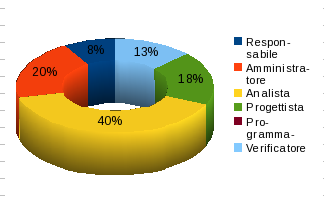
\includegraphics[width=300pt]{Cons-RR-RPP2}
\newpage

\begin{center}\textbf{Costo/Ruolo}
\end{center}
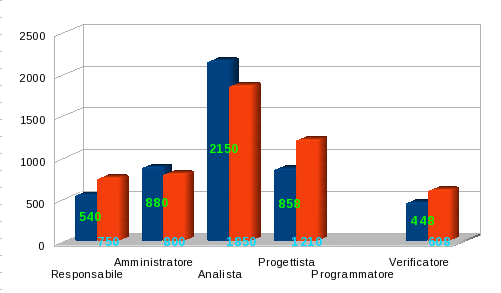
\includegraphics[width=350pt]{Cons-RR-RPP1}


\begin{table}[!h]
	\begin{center}
		  \begin{tabular}
			  {|c|c|c|c|c|c|c|c|}
		 \hline
%%%%%%%%%%%%%%INTESTAZIONE COLONNE%%%%%%%%%%%%%%%%%%%%%%%%%%%%%%%%%%%%%%%%%%%%%%%%%%%%%%%%%%%%%%
%			\multicolumn{3}{|c|}{ \multirow{2}{*}{ FASE RR - RPP } } \\
			\multicolumn{8}{|c|}{ \textbf{Consuntivo Ore/Ruolo} } \\
			\hline
			\textbf{Componente} & \multicolumn{7}{|c|}{ \textbf{RUOLO} } \\
			\hline
			& \textbf{Resp.} & \textbf{Amm.} & \textbf{Analis.} & \textbf{Progett.} & \textbf{Program.} & \textbf{Verif.}  & \textbf{Totale}\\
			\hline
%%%%%%%%%%%%%%FINE INTESTAZIONE COLONNE%%%%%%%%%%%%%%%%%%%%%%%%%%%%%%%%%%%%%%%%%%%%
								     %  RESP    % AMMIN  %  ANALISTA  %  PROGET. %  PROGRAM %    VERIF.   % TOTALE
			Bizzotto Piero &  6   &  13 &  0   &   26  &  0   &  0  &  45 \\ % R4
			\hline
			Carollo Mirko &  8   &  24  &  0  &  9   &  0   &  0   &  41\\ % R5
			\hline
			Cunico Marco    &  0   &  0  &  25   &  0   &  0  &  0   &  25\\ % R2
			\hline
			Dal Bosco Davide   &  2   &  0   &  9   &  0   &   0  &  0  &  11\\ % R1
			\hline
			Dissegna Stefano        &  0  &  0   & 23  &  0   &  0  &  0  &  23\\ % R6
			\hline
			Geremia Mirco   &   2  &  7   &  9  &  0  &  0   &  17   &  35\\ % R7
			\hline	
			Rizzo Maurizio  &  0  &  0  &  16  &  4  &  0  &  11  &  31 \\ %R3
			\hline	
%%%%%%%%%%% FINE PARTE DA MODIFICARE %%%%%%%%%%%%%%%%%%%%%%%%%%%%%%%%%%%
		\end{tabular}
	\caption{Consuntivo carico/persona RR-RPP} %INSERIRE DIDASCALIA - SE NECESSARIA - 
	\label{tab: ConsPersOre_RR-RPP}
	\end{center}	
\end{table}

Come si pu\`o vedere dai dati precendentemente elencati si sono rivelate necessarie alcune modifiche rispetto al preventivo presentato:
sono stati richiesti sforzi maggiori dal ruolo di amministratore per l'attuazione di piani e procedure di gestione della qualit\`a ed
analista per analizzare pi\`u a fondo i requisiti. I ruoli di responsabile, progettista e verificatore hanno invece richiesto minori
risorse del previsto anche grazie al buon lavoro svolto nella fase PRE-RR.

\newpage

\subsezione{Fase RPP-RQ}
\begin{table}[h]
	\begin{center}
		  \begin{tabular}{|c|c|c|c|}
		 \hline 
		 \textbf{Ruolo} & \textbf{Ore di lavoro} & \textbf{Costo in euro}\\
		 \hline
		Responsabile & 31 & 930 \\
		Amministratore & 42 & 840\\
		Analista & 12 & 300\\
		Progettista & 82 & 1804\\
		Programmatore & 103 & 1648 \\
		Verificatore & 97 & 1552\\
        \hline
        \textbf{Totale} & \textbf{367} & \textbf{7074}\\
		\hline
		\end{tabular}
	\caption{Consuntivo RPP-RQ} 
	\label{tab:cons_RPP-RQ}
	\end{center}	
\end{table}

\begin{center}\textbf{Ore/Ruolo}
\end{center}
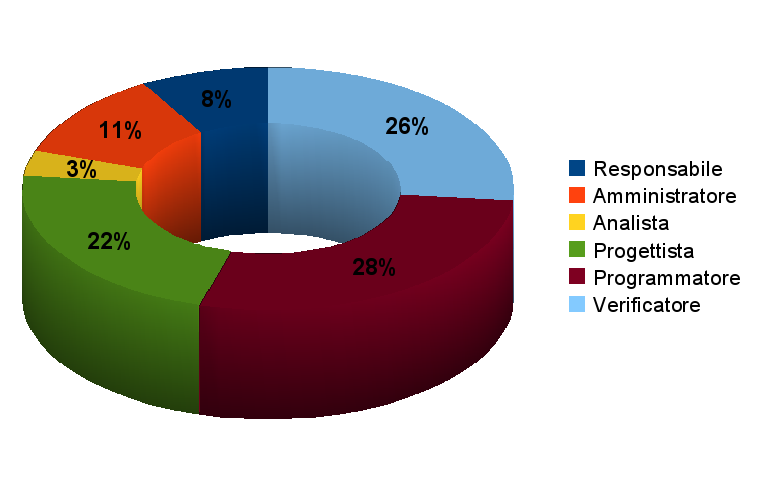
\includegraphics[width=300pt]{Cons-RPP-RQ1}
\newpage

\begin{center}\textbf{Costo/Ruolo}
\end{center}
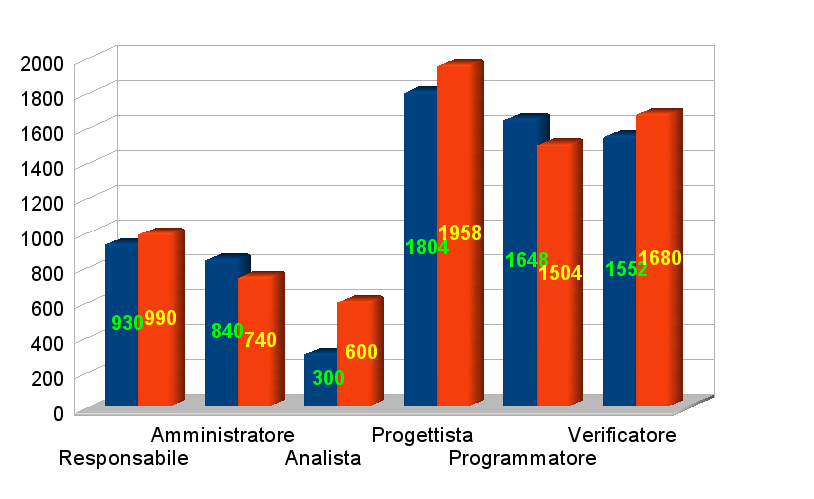
\includegraphics[width=350pt]{Cons-RPP-RQ2}


\begin{table}[!h]
	\begin{center}
		  \begin{tabular}
			  {|c|c|c|c|c|c|c|c|}
		 \hline
%%%%%%%%%%%%%%INTESTAZIONE COLONNE%%%%%%%%%%%%%%%%%%%%%%%%%%%%%%%%%%%%%%%%%%%%%%%%%%%%%%%%%%%%%%
%			\multicolumn{3}{|c|}{ \multirow{2}{*}{ FASE RPP - RQ} } \\
			\multicolumn{8}{|c|}{ \textbf{Consuntivo Ore/Ruolo} } \\
			\hline
			\textbf{Componente} & \multicolumn{7}{|c|}{ \textbf{RUOLO} } \\
			\hline
			& \textbf{Resp.} & \textbf{Amm.} & \textbf{Analis.} & \textbf{Progett.} & \textbf{Program.} & \textbf{Verif.}  & \textbf{Totale}\\
			\hline
%%%%%%%%%%%%%%FINE INTESTAZIONE COLONNE%%%%%%%%%%%%%%%%%%%%%%%%%%%%%%%%%%%%%%%%%%%%
							%RESP    % AMMIN  %  ANALISTA  %  PROGET. %  PROGRAM %    VERIF.   % TOTALE
			Bizzotto Piero 		&  0  &  0  &  4  &  0  &  13 &  28 &  45 \\ % R4
			\hline
			Carollo Mirko 		&  0  &  0  &  12 &  0  &  10 &  31 &  49\\ % R5
			\hline
			Cunico Marco    	&  7  &  11 &  0  &  23 &  16 &  0  &  57\\ % R2
			\hline
			Dal Bosco Davide   	&  8  &  5  &  0  &  16 &  11 &  38 &  78\\ % R1
			\hline
			Dissegna Stefano    &  8  &  10 &  0  &  20 &  23 &  0  &  61\\ % R6
			\hline
			Geremia Mirco   	&  0  &  0  &  0  &  23 &  18 &  0  &  41\\ % R7
			\hline	
			Rizzo Maurizio  	&  8  &  16 &  0  &  0  &  12 &  0  &  36\\ %R3
			\hline	
%%%%%%%%%%% FINE PARTE DA MODIFICARE %%%%%%%%%%%%%%%%%%%%%%%%%%%%%%%%%%%
		\end{tabular}
	\caption{Consuntivo carico/persona RPP-RQ} %INSERIRE DIDASCALIA - SE NECESSARIA - 
	\label{tab: ConsPersOre_RPP-RQ}
	\end{center}	
\end{table}

Si pu\`o notare dai dati che in generale \`e stato richiesto un impegno leggermente minore rispetto a quanto previsto, in particolare il ruolo di Analista ha richiesto meno impegno, poich\`e nel preventivo l'azienda si era tutelata su questo campo inserendo ore extra per eventuali problemi. Sono state utilizzate meno ore anche per quel che riguarda la verifica, dove hanno giocato un ruolo importante gli stumenti adottati e le modalit\`a di automazione della gestione degli errori, che hanno permesso di velocizzare i processi di verifica. L'unico ruolo che ha richiesto un maggiore impegno \`e stato quello del Programmatore, poich\`e si sono riscontrati problemi non previsti nell'implementazione di alcuni elementi.

\subsubsezione{Implicazioni del consuntivo}
In questa fase il progetto \`e in fase di completamento e ci si aspetta un lavoro nella fase seguente per quel che riguarda la codifica e la relativa verifica. Il preventivo relativo alla fase RQ-RA \`e stato quindi aggiornato per questo motivo, e soprattutto per l'acquisizione e l'integrazione di un nuovo membro all'interno dell'azienda.

\newpage

\subsezione{Fase RQ-RA}
\begin{table}[h]
	\begin{center}
		  \begin{tabular}{|c|c|c|c|}
		 \hline 
		 \textbf{Ruolo} & \textbf{Ore di lavoro} & \textbf{Costo in euro}\\
		 \hline
		Responsabile & 10 & 300 \\
		Amministratore & 13 & 260\\
		Analista & 0 & 0\\
		Progettista & 11 & 242\\
		Programmatore & 17 & 272\\
		Verificatore & 26 & 416\\
        \hline
        \textbf{Totale} & \textbf{77} & \textbf{1490}\\
		\hline
		\end{tabular}
	\caption{Consuntivo RQ-RA} 
	\label{tab:cons_RPP-RQ}
	\end{center}	
\end{table}

\begin{center}\textbf{Ore/Ruolo}
\end{center}
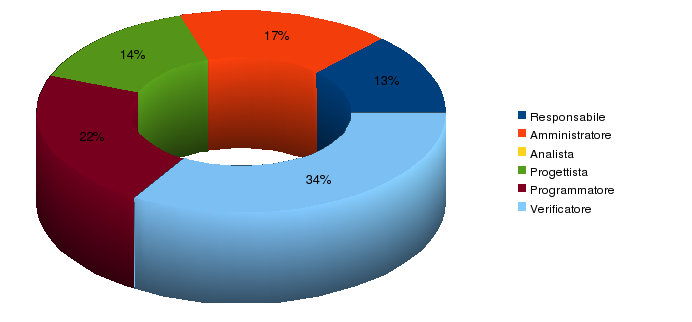
\includegraphics[width=300pt]{Cons-RQ-RA1}
\newpage

\begin{center}\textbf{Costo/Ruolo}
\end{center}
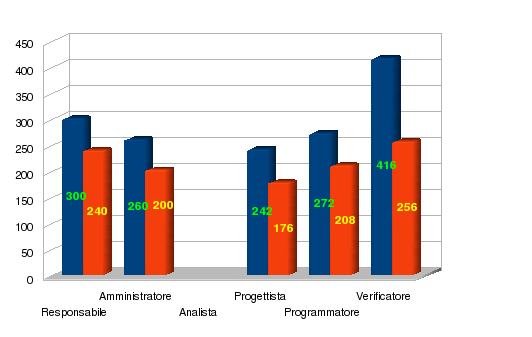
\includegraphics[width=350pt]{Cons-RQ-RA2}


\begin{table}[!h]
	\begin{center}
		  \begin{tabular}
			  {|c|c|c|c|c|c|c|c|}
		 \hline
%%%%%%%%%%%%%%INTESTAZIONE COLONNE%%%%%%%%%%%%%%%%%%%%%%%%%%%%%%%%%%%%%%%%%%%%%%%%%%%%%%%%%%%%%%
%			\multicolumn{3}{|c|}{ \multirow{2}{*}{ FASE RQ - RA} } \\
			\multicolumn{8}{|c|}{ \textbf{Consuntivo Ore/Ruolo} } \\
			\hline
			\textbf{Componente} & \multicolumn{7}{|c|}{ \textbf{RUOLO} } \\
			\hline
			& \textbf{Resp.} & \textbf{Amm.} & \textbf{Analis.} & \textbf{Progett.} & \textbf{Program.} & \textbf{Verif.}  & \textbf{Totale}\\
			\hline
%%%%%%%%%%%%%%FINE INTESTAZIONE COLONNE%%%%%%%%%%%%%%%%%%%%%%%%%%%%%%%%%%%%%%%%%%%%
							%RESP    % AMMIN  %  ANALISTA  %  PROGET. %  PROGRAM %    VERIF.   % TOTALE
			Bizzotto Piero 		&  2  &  6  &  0  &  0  &  0 &  0 &  8 \\ % R4
			\hline
			Carollo Mirko 		&  0  &  0  &  0 &  0  &  0 &  2 &  2\\ % R5
			\hline
			Cunico Marco    	&  0  &  5 &  0  &  0 &  8 &  3  &  16\\ % R2
			\hline
			Dal Bosco Davide   	&  0  &  2  &  0  &  0 &  6 &  0 &  8\\ % R1
			\hline
			Dissegna Stefano    &  8  &  0 &  0  &  2 &  0 &  3  &  13\\ % R6
			\hline
			Geremia Mirco   	&  0  &  0  &  0  &  9 &  3 &  0  &  12\\ % R7
			\hline	
			Rizzo Maurizio  	&  0  &  0 &  0  &  0  &  0 &  18  &  18\\ %R3
			\hline	
%%%%%%%%%%% FINE PARTE DA MODIFICARE %%%%%%%%%%%%%%%%%%%%%%%%%%%%%%%%%%%
		\end{tabular}
	\caption{Consuntivo carico/persona RQ-RA} %INSERIRE DIDASCALIA - SE NECESSARIA - 
	\label{tab: ConsPersOre_RPP-RQ}
	\end{center}	
\end{table}

Si pu\`o notare dai dati che in generale \`e stato richiesto un impegno maggiore rispetto a quanto previsto.
In questa fase finale \`e stato completato lo sviluppo del progetto, sono stati prodotti l'utilit\`a di installazione e il manuale utente (gi\`a iniziato nella scorsa fase). Il resto del tempo e delle risorse residue sono state impiegate nel processo di qualifica.

\newpage
\sezione{Consuntivo di fine progetto}
Viene presentato in questa sezione il consuntivo al termine della fase
di sviluppo del progetto AJAXDRAW, da parte di WebShape. In tabella \ref{tab:ConsCaricoFase_Totale} vengono mostrati i dati consuntivi delle ore dell'intero svolgimento
del progetto divise per fase.

\begin{table}[!h]
	\begin{center}
		  \begin{tabular}
			  {|c|c|c|c|c|c|c|c|}
		 \hline
%%%%%%%%%%%%%%INTESTAZIONE COLONNE%%%%%%%%%%%%%%%%%%%%%%%%%%%%%%%%%%%%%%%%%%%%%%%%%%%%%%%%%%%%%%
%			\multicolumn{3}{|c|}{ \multirow{2}{*}{ FASE RQ - RA} } \\
			\multicolumn{6}{|c|}{ \textbf{Consuntivo Ore/Ruolo divise per fase} } \\
			\hline
			 & \multicolumn{4}{|c|}{ \textbf{FASI} } & \\
			\hline
			\textbf{Ruolo} & \textbf{RR-RPP} & \textbf{RPP-RQ} & \textbf{RQ-RA} & \textbf{Totale} & \textbf{Scostamento}\\
			\hline
%%%%%%%%%%%%%%FINE INTESTAZIONE COLONNE%%%%%%%%%%%%%%%%%%%%%%%%%%%%%%%%%%%%%%%%%%%%
			Responsabile 		&  18  &  31  &  10  &  59  & -7\\ % R4
			\hline
			Amministratore 		&  44  &  42  &  13 &  99 & -12\\ % R5
			\hline
			Analista   	&  86  &  12 &  0  &  98 & 0\\ % R2
			\hline
			Progettista   	&  39  &  82  &  11  &  132 & -20\\ % R1
			\hline
			Programmatore    &  0  &  103 &  17  &  120 & +13\\ % R6
			\hline
			Verificatore   	&  28  &  97  &  26  &  151 & -8\\ % R7
			\hline		
%%%%%%%%%%% FINE PARTE DA MODIFICARE %%%%%%%%%%%%%%%%%%%%%%%%%%%%%%%%%%%
		\end{tabular}
	\caption{Consuntivo carico/fase Totale} %INSERIRE DIDASCALIA - SE NECESSARIA - 
	\label{tab:ConsCaricoFase_Totale}
	\end{center}	
\end{table}
%%%Costo in Euro   	&  4876  &  7074  &  1490  &  13440\\ % R7

\begin{center}\textbf{Ore/Ruolo}
\end{center}
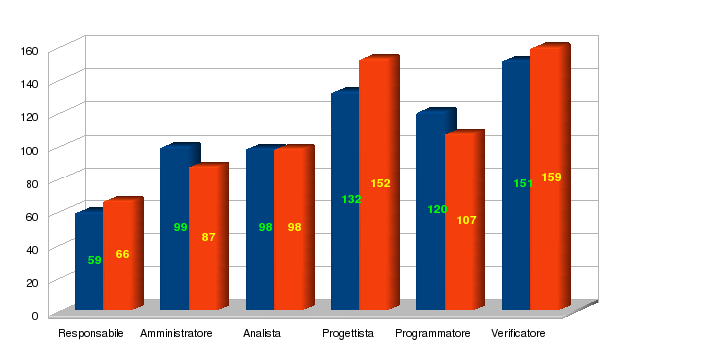
\includegraphics[width=420pt]{Cons-Ore-Totale}

\newpage
\begin{center}\textbf{Costo/Ruolo}
\end{center}
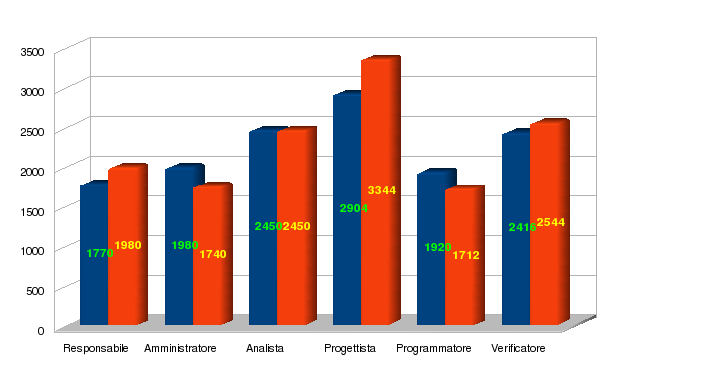
\includegraphics[width=420pt]{Cons-Costi-Totale}

\begin{table}[h]
	\begin{center}
		  \begin{tabular}{|c|c|c|c|}
		 \hline 
		 \textbf{Ruolo} & \textbf{Ore di lavoro} & \textbf{Costo in euro}\\
		 \hline
		Responsabile & 59 & 1770 \\
		Amministratore & 99 & 1980\\
		Analista & 98 & 2450\\
		Progettista & 132 & 2904\\
		Programmatore & 120 & 1920\\
		Verificatore & 151 & 2416\\
        \hline
        \textbf{Totale} & \textbf{659} & \textbf{13440}\\
		\hline
		\textbf{Scostamento} & \textbf{-10} & \textbf{-330} \\	\hline
		\end{tabular}
	\caption{Consuntivo Totale} 
	\label{tab:cons_Totale}
	\end{center}	
\end{table}

Anche se nel corso dell'intero progetto sono state necessarie delle variazioni per quanto
riguarda la pianificazione del lavoro, \`e stato comunque possibile mantenere i costi
bassi, in relazione :
\begin{elenconumerato}{\normindent}
				\item al non superamento dei costi preventivi realizzati nella presentazione dell'offerta
				\item al soddisfacimento delle funzionalit\`a richieste al prodotto, poste durante la fase di
       analisi dei requisiti
\end{elenconumerato}

\newpage
\begin{table}[!h]
	\begin{center}
		  \begin{tabular}
			  {|c|c|c|c|c|c|c|c|}
		 \hline
%%%%%%%%%%%%%%INTESTAZIONE COLONNE%%%%%%%%%%%%%%%%%%%%%%%%%%%%%%%%%%%%%%%%%%%%%%%%%%%%%%%%%%%%%%
%			\multicolumn{3}{|c|}{ \multirow{2}{*}{ FASE RQ - RA} } \\
			\multicolumn{8}{|c|}{ \textbf{Consuntivo Ore/Ruolo} } \\
			\hline
			\textbf{Componente} & \multicolumn{7}{|c|}{ \textbf{RUOLO} } \\
			\hline
			& \textbf{Resp.} & \textbf{Amm.} & \textbf{Analis.} & \textbf{Progett.} & \textbf{Program.} & \textbf{Verif.}  & \textbf{Totale}\\
			\hline
%%%%%%%%%%%%%%FINE INTESTAZIONE COLONNE%%%%%%%%%%%%%%%%%%%%%%%%%%%%%%%%%%%%%%%%%%%%
							%RESP    % AMMIN  %  ANALISTA  %  PROGET. %  PROGRAM %    VERIF.   % TOTALE
			Bizzotto Piero 		&  8  &  19  &  4  &  26  &  13 &  28 &  98 \\ % R4
			\hline
			Carollo Mirko 		&  8  &  24  &  12 &  9  &  10 &  33 &  96\\ % R5
			\hline
			Cunico Marco    	&  7  &  16 &  25  &  23 &  24 &  3  &  98\\ % R2
			\hline
			Dal Bosco Davide   	&  10  &  7  &  9  &  16 &  17 &  38 &  97\\ % R1
			\hline
			Dissegna Stefano    &  16  &  10 &  23  &  22 &  23 &  3  &  97\\ % R6
			\hline
			Geremia Mirco   	&  2  &  7  &  9  &  32 &  21 &  17  &  88\\ % R7
			\hline	
			Rizzo Maurizio  	&  8  &  16 &  16  &  4  &  12 &  29  &  85\\ %R3
			\hline	
%%%%%%%%%%% FINE PARTE DA MODIFICARE %%%%%%%%%%%%%%%%%%%%%%%%%%%%%%%%%%%
		\end{tabular}
	\caption{Consuntivo carico/persona Totale} %INSERIRE DIDASCALIA - SE NECESSARIA - 
	\label{tab: ConsPersOre_Totale}
	\end{center}	
\end{table}

\begin{center}\textbf{Distribuzione Componenti}
\end{center}
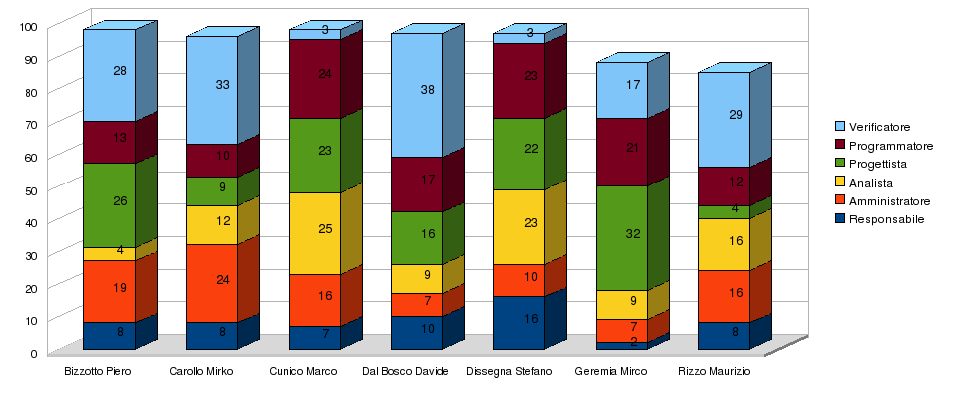
\includegraphics[width=420pt]{Cons}


\end{document}
